\documentclass[conference]{IEEEtran}
\IEEEoverridecommandlockouts
% The preceding line is only needed to identify funding in the first footnote. If that is unneeded, please comment it out.
\usepackage{cite}
\usepackage{amsmath,amssymb,amsfonts}
\usepackage{algorithmic}
\usepackage{graphicx}
\usepackage{textcomp}
\usepackage{xcolor}
\def\BibTeX{{\rm B\kern-.05em{\sc i\kern-.025em b}\kern-.08em
    T\kern-.1667em\lower.7ex\hbox{E}\kern-.125emX}}
\begin{document}

\title{Distributed Systems - Surveillance System Project}

\author{\IEEEauthorblockN{1\textsuperscript{st} Cedric Sillaber}
\and
\IEEEauthorblockN{2\textsuperscript{nd} Alan Gallo}
\and
\IEEEauthorblockN{3\textsuperscript{rd} Frantisek Sova}
}
%TODO: explain new async.queue for edge: queue collects data, and asynchronous worker processes it

\maketitle

\section{Introduction}
In our surveillance system, cameras are simulated using the WiseNET dataset. The system is designed to capture video streams and process them efficiently for real-time object and facial recognition. The video data undergoes preprocessing at the edge, minimizing the workload on the cloud, reducing latency, and optimizing the overall performance of the surveillance system. The system leverages edge devices and cloud services to ensure scalability, fast response times, and effective monitoring.  

\section{System architecture}
The video files are stored in camera containers running on a single EC2 instance \ref{fig:architecture}. Each container parses a certain video file into images using OpenCV. These sequences are then sent to edge devices at regular intervals through HTTP, simulating a real-time video stream. Communication between components is handled through a WebSocket, which is capable of managing large payloads and scaling efficiently. Additionally, the EC2 instance houses an alarm container, completing the IoT layer of the system.

\begin{figure}[h!]
    \centering
    %\includegraphics[width=1\linewidth]{res/report/DS_architecture_version2.png}
    \includegraphics[width=1\linewidth]{DS_architecture_version2.png}
    \caption{Example of your architectural diagram.}
    \label{fig:architecture}
\end{figure}

The edge layer consists of a single EC2 instance simulating edge devices in different locations. At the edge, the video data is processed using the YOLO (You Only Look Once) algorithm to detect objects and people. When a person-like object is detected, the relevant data is forwarded to a separate instance in the cloud, ensuring the system can scale dynamically based on demand.

The cloud layer integrates with Amazon Rekognition to perform facial recognition, comparing the detected face against a collection of known individuals. If an unknown person is identified, the cloud server triggers an alert, which is sent back to the edge device and activates the alarm in the IoT layer. This architecture reduces the workload on the cloud, minimizes latency, and ensures the system can handle large volumes of video data in a responsive and efficient manner, making it a robust solution for surveillance applications.



\section{Implementation details}
Our implementation consists of three distinct layers: IoT, Edge, and Cloud, each with specific responsibilities and components.

\subsection{IoT Layer}
The IoT layer consists of 4 camera containers and one alarm container for each edge device. We utilize the WiseNET dataset (set\_3) for video simulation, which features two individuals appearing at different times in the scene - one simulating an intruder and another an employee. The camera containers are designed to have access to the complete set of videos, though each container selects only one based on a container-specific environment variable \textit{CAMERA}. The video sets are \textit{.avi-files} that are read sequentially and looped when the end is reached. 
These videos are processed using OpenCV's read() function to extract frame sequences. The system then transmits these frames to the edge device using Socket.IO library at intervals that simulate real-time frame rates. The alarm container maintains a connection to the edge server and remains in a waiting state until triggered by an event.

\subsection{Edge Layer}
The edge layer operates as an EC2 instance running the YOLO (You Only Look Once) algorithm for object detection. The implementation is Python-based and utilizes OpenCV for frame processing. Images from the IoT layer are received by the edge device using the Socket.IO library. When the system detects a person-like object using YOLO, it immediately forwards the relevant data to the cloud server through a REST API interface.

\subsection{Cloud Layer}
The cloud implementation centers around facial recognition and alert management through a REST API built using Python's Flask package to receive images from the edge layer. The system integrates directly with AWS Rekognition for facial recognition processing, with automatic provisioning of the Rekognition collection and known faces occurring at cloud server startup using boto3. When processing is complete, the result is returned in the HTTP response. Upon detection of an unknown person, the system triggers an alert, informs the edge layer through the HTTP response, and activates the appropriate alarm.

The system assumes a network topology where multiple cameras at a single location connect to one edge device. Each edge device manages multiple cameras but only one alarm. The cloud layer is designed to handle multiple edge devices simultaneously, with the capability to trigger location-specific alarms when intruders are detected.


\subsection{Implementation Decisions}
In the software stack where several options were available and we decided to go for specific ones. This section provides rationale for the choices made. This includes the programming language, communication libraries and detection algorithms.
\\

\subsubsection{Communication}
The distributed system consists of several components that need to communicate in an efficient way - that's what makes it a distributed system. 
Namely two main interfaces need communictation:
\\
\begin{itemize}
    \item IOT - Edge communication
    \item Edge - Cloud communication
\end{itemize}

\hfill \break
For the \textbf{IOT - Edge} communication we decided to use socket.io. This Python library enables communication with websockets. As we need to send a constant stream of data, this communication model seems to be the best fit. The protocol includes a full-duplex communication channel build ontop of the network layer. Its a consistent communication model that requires minimal overhead for setting up the connection. 

This model handles many frames transfered very well and is very efficient. In comparision to HTTP that would require a new connection for every frame, this model is much more efficient. 
\\

%TODO: insert example of socket.io communication wit sockets.

For the \textbf{Edge - Cloud} communication we decided to use a REST API. This approach was implemented using Python's \textit{Flask} package to allow the distributed processing of the data. 

Our assumption for the choice of the communication model was that the data transfer between Edge and Cloud is not as frequent as between IOT and Edge. Ideally only a few requests per hour are sent to the cloud, as there are only few intruders in the office. When we would have tens of thousands of requests to the server per minute, we would argue there is something wrong in the office. 

Given our assumption, the overhead of setting up a new connection for every request is not as significant. Having a constant connection open to the cloud would be a waste of resources. 

The REST API is a stateless communication model that uses HTTP requests to transfer data. It is simple to implement and easy to understand. 

Whenever the preprocessing model (YOLO) detects a person in a frame, it sends the frame in a HTTP request to the cloud for further processing. 
The cloud immediately processes the image and sends the response back in the HTTP response. We efficiently use the request and respons for our computation. 
\hfill \break

\subsubsection{Dection Models}
In the system two detection models are used, namely: 
\begin{itemize}
\item YOLO: preprocessing images on Edge
\item AWS Rekognition: facial recognition on Cloud
\end{itemize}

\hfill \break

It was obvious to us to use Rekognition, as we already tested this AWS service in the course of the semester. It is a very powerful tool for facial recognition and very easy to use. 

YOLO was chosen as the detection model for the edge, as it is a very efficient object detection model. It is able to process images in real-time and is very accurate. There were multiple problems in setting up the model in Docker, especially with dependencies for the \textit{pytorch} library. We found a workaround using \textit{ultralytics} package, that wrappes \textit{torch} and special classes for YOLO into one package. Unfortunately the package is exceptionally big and exceeds the maximum image size of 1GB. We had no time to further optimize the size of the edge layer and decided to use the large image. 

YOLO and Rekognition can be easily encapsulated and used in the system. 
For example, we implemented a wrapper class for yolo usage, so we can use simply the \textit{yoloDetection.analyseImage(image)} function. 
Internally this function runs the yolo image detection, and returns True if a person was detected, otherwise False. 

\begin{center}
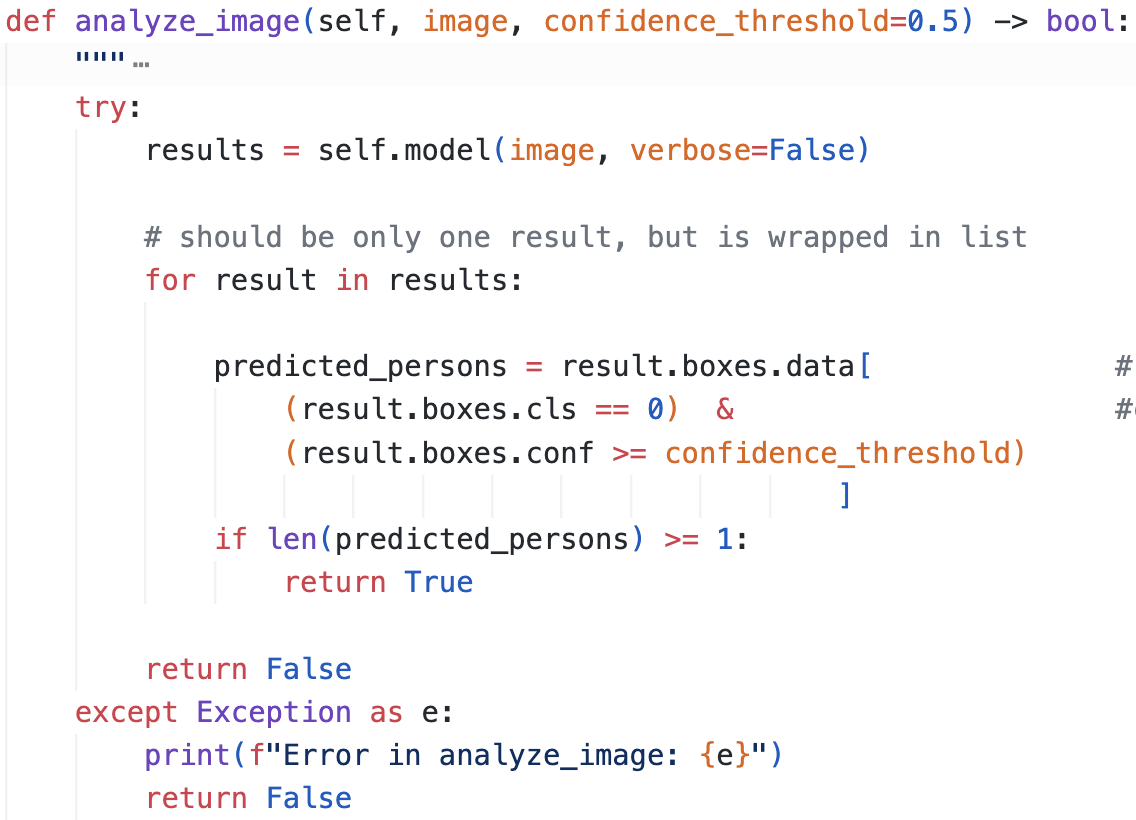
\includegraphics[width=1\linewidth]{analyze_image-function.png}
\end{center}

\section{Testing Setup}
In the first weeks of implementing the distributed system, we solely focused on simulating disjoint networks in Docker, utilizing the Docker-Networks feature. 

For every layer, we created a separate Dockerfile.[layer]. A simple \texttt{docker-compose.yaml} file was used to orchestrate the containers. In this orchestration, the camera containers were connected to the edge device, which in turn was connected to the cloud server. 
The IOT containers are connected to the same network as the edge, the edge in addition is connected to the cloud network. 
The following \textit{.yaml} shows the configuration for networking in docker containers.

\begin{verbatim}
networks:
  simulation_network:
    driver: bridge
  simulation_network_edge_cloud:
    driver: bridge

# then in the container specification: 
cloud: 
    build:
    context: .
    dockerfile: docker/Dockerfile.cloud
    image: cloud
    networks:
    # subscribe to the network
    - simulation_network_edge_cloud 
\end{verbatim}

This simple setup allowed us to test the communication between the layers and the correct processing of the data. 
Deployment was easy then, just a matter of spinning up the containers on the EC2 instances and adapting the IP addresses in the config file.

\section{Deployment Setup}
The entire distributed system runs on three AWS EC2 instances:
\begin{itemize}
    \item IOT - layer: camera instances
    \item EDGE - layer: edge instance with YOLO
    \item CLOUD - layer: cloud instance with AWS Rekognition
\end{itemize}

\hfill \break

The IoT layer components (4 camera containers and 1 alarm container) are consolidated on a single t2.micro instance, which is sufficient for simulating the video streams and alarm functionality.

The edge layer operates on a t2.medium instance. This increased computational capacity is necessary due to the resource demands of the YOLO algorithm for real-time person detection.

The cloud layer, hosting the AWS Rekognition integration and REST API, runs on a t2.micro instance, as the facial recognition processing is offloaded to AWS services.

This deployment configuration provides a cost-effective setup while ensuring adequate processing power where needed, particularly for the computationally intensive edge layer operations.

\begin{figure}[h!]
    \centering
    %\includegraphics[width=1\linewidth]{res/report/DS_architecture_version2.png}
    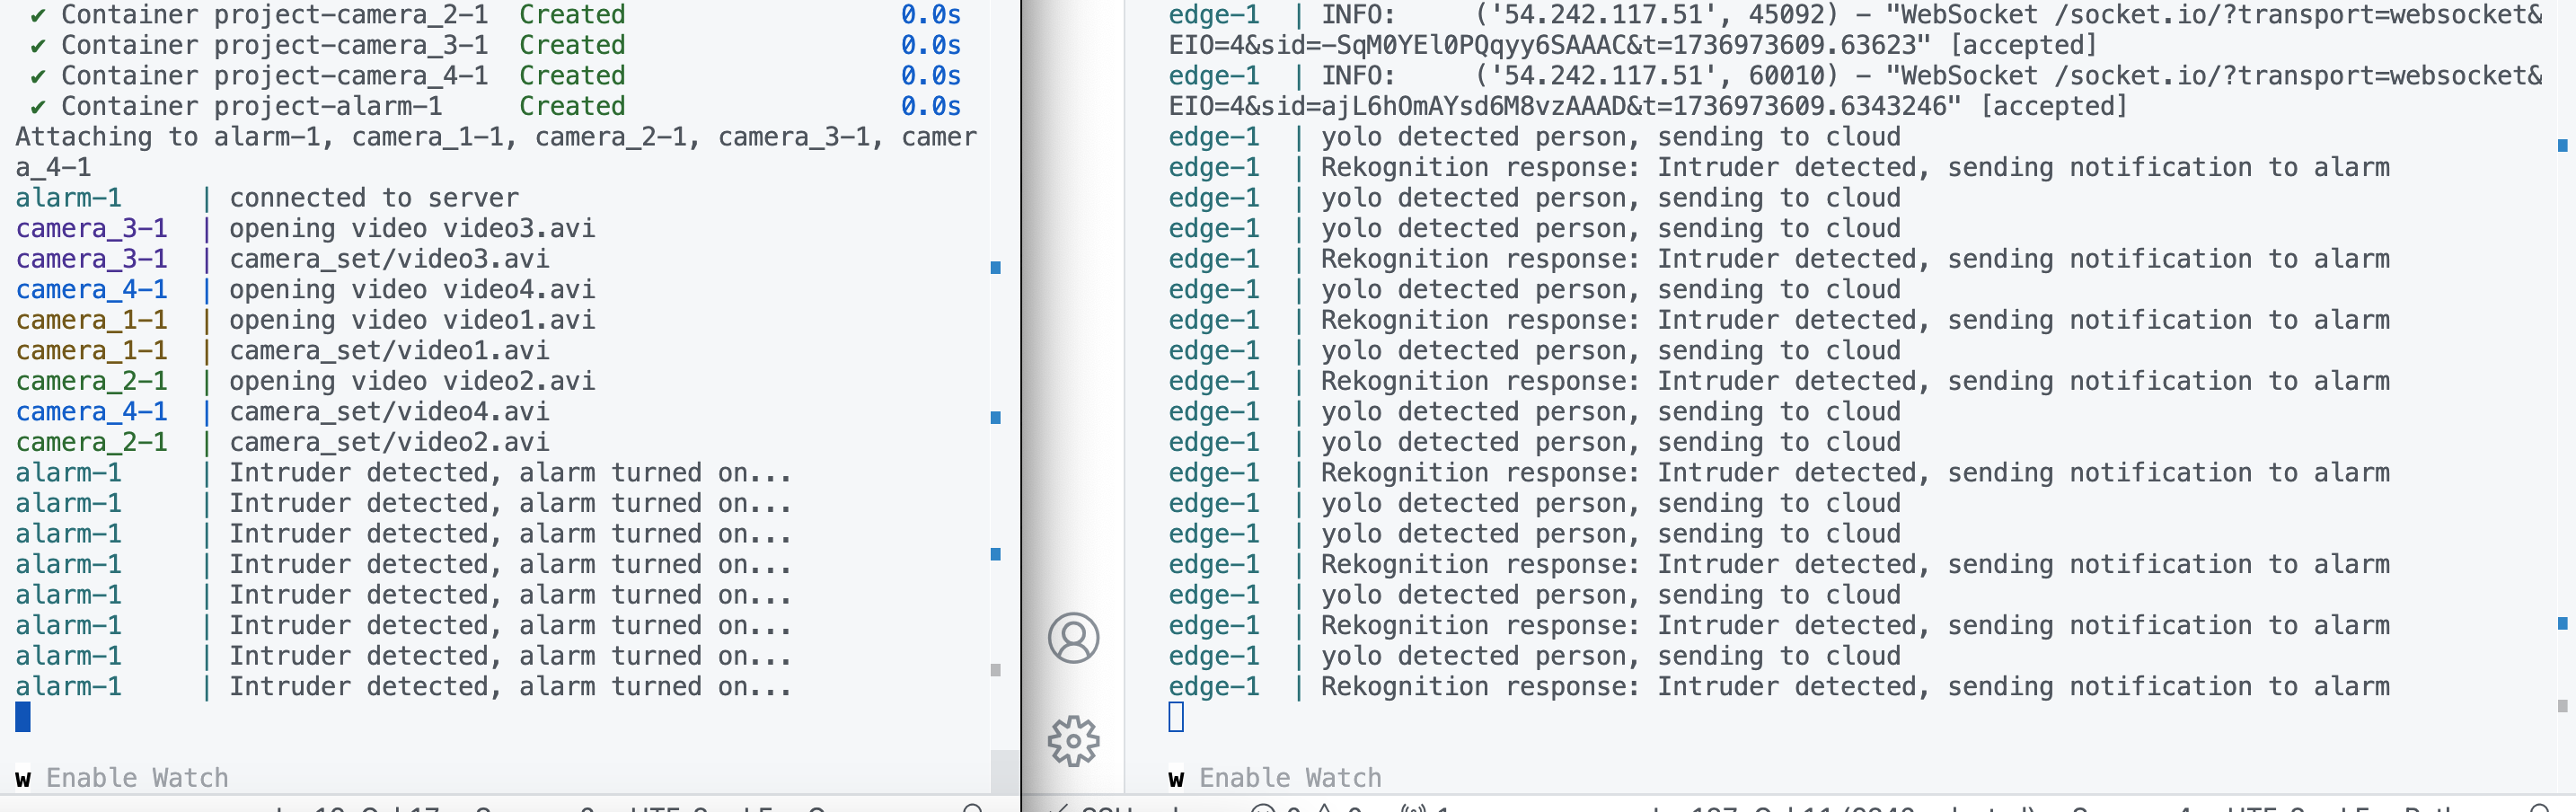
\includegraphics[width=1\linewidth]{deployment2.png}
    \caption{Sucessful detection of intruders.}
    \label{fig:deployment}
\end{figure}
\section{Evaluation}
Evaluation of the response time and scalability (number of devices and traffic) to prove the correctness of your implementation. The more detailed the better. 

\end{document}
